\chapter{Erosion}
\label{chap:erosion}

\section{Introduction}
\label{sec:intro}
Solid body erosion can be seen in every day life in various physical processes.
It is commonly seen in areas where solid particles are carried in a pipe, body
part erosion of an aircraft due to high speed impact of particles. Due to the
continuous erosion, the conveying systems can result in total damage and failure
of the manufacturing system. Similarly, the aerodynamic performance of the wings
as well as other parts of an aircraft may reduce. An accurate study of the solid
particle erosion can be helpful in improving the life and efficiency of such
systems and reduce the maintenance cost. Experimental investigation is complex.
Also, the experimental investigation will not give insight into the details of
the erosion process.


In the current chapter we model the solid particle erosion of a ductile target.
We utilise the developments done to this point. Handling of collision between
the rigid bodies, elastic bodies and modeling of elastic structure in
\cref{chap:ctvf,chap:csph,chap:ctvf} is utilized. We develop a numerical method
to simulate elastic-plastic solids. The current scheme is able to eliminate
several issues in classic SPH method. A contact force model is used to handle
the collision between the impactor and the target. The developed technique is
further applied to handle rigid fluid coupling as well as to model fluid
structure interaction problems. Finally, an elastic-plastic algorithm is
incorporated in the new scheme to model the solid particle erosion. The complete
work is made open source and is fully reproducible.



\FloatBarrier%
\section{Numerical method}
\label{sec:erosion-numerical-method}
In the current section we write the equations governing the behaviour
elastic-plastic target. We utilise the scheme developed in \cref{chap:ctvf} to
model the elastic solids, to which we add additional equations to consider the
plastic behaviour. We employ the equations used in \cref{chap:rfc} to model the
dynamics of the rigid bodies as well as their interaction. From \cref{chap:csph}
and \cref{chap:rfc}, we develop a contact force formulation and adapt it to
handle the contact between the rigid and an elastic-plastic body.

\subsection{Discrete governing equations of the ductile target}
\label{chap-erosion:sec:discrete-governing-equations}
In addition to the equations of an elastic solid in
\cref{sec:ctvf-sph-equations}, i.e., continuity and momentum, we consider
energy equation to track the temperature of the solid particles. While the
momentum equation is modified to consider the contact due to the external
impact. The new set of equations are,
\begin{figure}[!htpb]
  \centering
  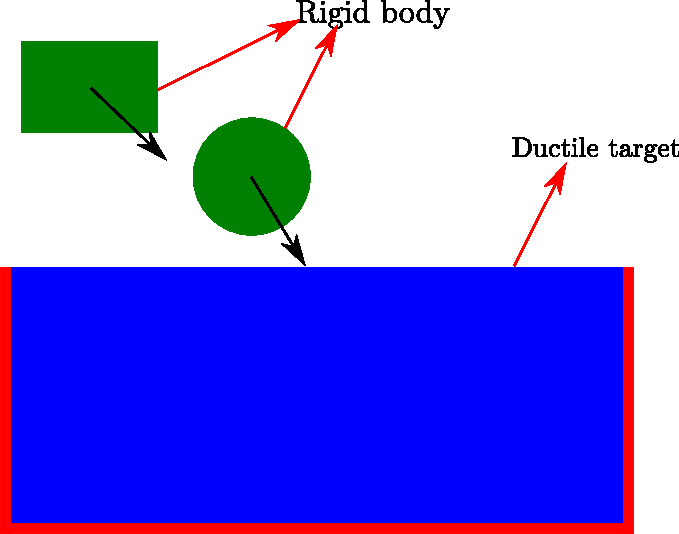
\includegraphics[width=0.5\textwidth]{images/erosion/images/intro/intro_description}
  \caption{Bodies under collision which are divided into primary and
    secondary.}
\label{fig:bodies_under_collision}
\end{figure}
\begin{eqnarray}
\label{eqn:erosion-sph-momentum}
  \frac{\tilde{d}\ten{u}_{a}}{dt} &=& - \sum_{b \in A} m_b \left[
  \left(\frac{p_a}{\rho_a^2} + \frac{p_b}{\rho_b^2}\right) \ten{I} -
  \left(\frac{\teng{\sigma}^{'}_{a}}{\rho_a^2} +
  \frac{\teng{\sigma}^{'}_{b}}{\rho_b^2} + \Pi_{ab} \ten{I} \right) \right]  \cdot \nabla_{a} W_{ab} +
  \ten{g}_{a} + \frac{1}{m_a}\sum_{b \in B} \ten{F}^{\text{cont}}_{a \leftarrow b},\\
  \frac{\tilde{d}{e}_{a}}{dt} &=& - \frac{1}{2} \sum_{b \in A} m_b
  \left(\frac{p_a}{\rho_a^2} + \frac{p_b}{\rho_b^2} + \Pi_{ab} \right)
  \left( \ten{v}_a - \ten{v}_b \right) \cdot \nabla_{a} W_{ab} +
  \frac{1}{\rho_a} \teng{\sigma}^{'}_{a} \rvdot \teng{\epsilon_a}.
\end{eqnarray}
Here, $\ten{F}^{cont}_{a}$ is the force acting on particle $a$ due to contact
with the other impacting rigid bodies which will be discussed in
\cref{chap-erosion:sec:rigid-body-collision}. The boundary conditions, particle position
evolution are similar to \cref{chap:ctvf}. These equations are combined
with von-Mises flow criterion to model the plasticity as described below.

We consider Johnson-Cook constitutive law to compute the flow stress of the
ductile body. Johnson-Cook model accounts for the effects of strain hardening,
strain rate hardening, and thermal softening. The flow stress is computed using
\begin{equation}
  \sigma_y = \bigg[A + B (\epsilon^{p}_{eff})^N \bigg]
  \bigg[1 + C \ln\bigg(\frac{\dot{\epsilon^{p}_{eff}}}{\dot{\epsilon_0}}\bigg) \bigg] \bigg[1 - (T^*)^M \bigg],
\end{equation}
where,
\begin{equation}
  \dot{\epsilon^{p}_{eff}} = \sqrt{\dot{\epsilon}_{\alpha \beta} \dot{\epsilon}_{\alpha \beta}},
\end{equation}
$A, B, N, \dot{\epsilon_{0}}, C, M$ are the Johnson-Cook parameters. $T^*$ is given as
\begin{equation}
  T^* = \frac{T - T_{ref}}{T_{melt} - T_{ref}},
\end{equation}
where $T_{ref}, T_{melt}, T$ are the room temperature, and melting point
temperature. $T$ is the temperature of the particle evolved using an energy
equation. The stress of the particle is adjusted in the integrator step (see
\cref{sec:time-integration}). The trial deviatoric stress $\sigma^{'}^{*}_{\alpha \beta}$
at the next time step is given as,
\begin{equation}
  \sigma^{'}^{*}_{\alpha \beta} = \sigma^{'}^{n}_{\alpha \beta} + \bigg( \frac{d\sigma^{'}}{dt}\bigg)_{\alpha \beta}  \; dt
\end{equation}
By using the flow stress computing using the Johnson-Cook model, we check if
the trial stress exceeds the yield value, which in case will be bought back to
the limit using the following equations,
\begin{equation}
  f_y = \min{(\sigma_y / \sigma^{'}^*, 1)}.
\end{equation}
where $\sigma^{'}^* = \sqrt{\frac{3}{2} \sigma^{'}^*_{ij} \sigma^{'}^*_{\alpha \beta}}$.
\begin{equation}
  \sigma^{'}^{n+1}_{\alpha \beta} = \hat{f} \; \sigma^{'}^{*}_{\alpha \beta}
\end{equation}

Finally, the new stress state is computed as
\begin{equation}
  \sigma^{n+1}_{\alpha \beta} = - P^{n+1}\delta_{\alpha \beta} + \sigma^{'}^{n+1}_{\alpha \beta}
\end{equation}
Similarly, the plastic strain increment is given by
\begin{equation}
  \Delta \epsilon^{p}_{\alpha \beta} = (1 - \hat{f}) \sigma^{'}^{*}_{\alpha \beta} / 2 \mu,
\end{equation}
and the effective plastic strain increment is computed as,
\begin{equation}
  \Delta \epsilon^{p} = \frac{1}{3} \frac{1 - \hat{f}}{\mu}\sigma^{'}^{*}
\end{equation}


\begin{equation}
  \epsilon_{\text{failure}} = [D_1 + D_2 \exp(D_3 \sigma^{*})]
  \bigg[ 1 + D_4 ln\big(\frac{\dot{\epsilon}_{eff}^p}{\dot{\epsilon}_{0}})\bigg]
  [1 + D_5 T^*]
\end{equation}

\begin{equation}
  D = \sum\frac{\Delta \epsilon_{eff}^p}{\epsilon_{\text{failure}}}
\end{equation}



\subsection{Rigid body dynamics}
\label{chap-erosion:sec:rigid-body-dynamics}
Following \cite{chap-rfc}, the governing equations of the rigid body are,
\begin{equation}
  \label{eq:balance_linear_mom}
  \frac{d \; (M \ten{v}_{cm})}{d t} = \sum_i \ten{F}_i,
\end{equation}
\begin{equation}
  \label{eq:balance_angular_mom}
  \frac{d \ten{L}}{d t} = \teng{\tau}
\end{equation}
where $\ten{F}_a = \ten{F}^{RB}_a + \ten{F}^{DS}_a$ are due to the interaction
with other rigid bodies ($\ten{F}^{RB}_a$) and the ductile
solid($\ten{F}^{DS}_a$). Force due to the other rigid bodies ($\ten{F}^{RB}_a$)
is computed using the formulation provided in \cite{sec:rfc:contact force} while
the force between the rigid body and the ductile solid is shown in
\cref{chap-erosion:sec:rigid-body-dynamics}.


\subsection{Contact force law}
\label{chap-erosion:sec:rigid-body-collision}

Following \cref{sec:contact-algorithm,rfc:sec:contact-algorithm}, we compute the
forces on the ductile body as well as the rigid body. In the current case we
consider the ductile body as the primary body and the rigid projectile as
secondary. This is due to the fact that the boundary particles of the rigid body
remains constant while the ductile target undergoes erosion and the surface
particles needs to be recomputed at every time instant if the target erodes.
\begin{figure}[!htpb]
  \centering
  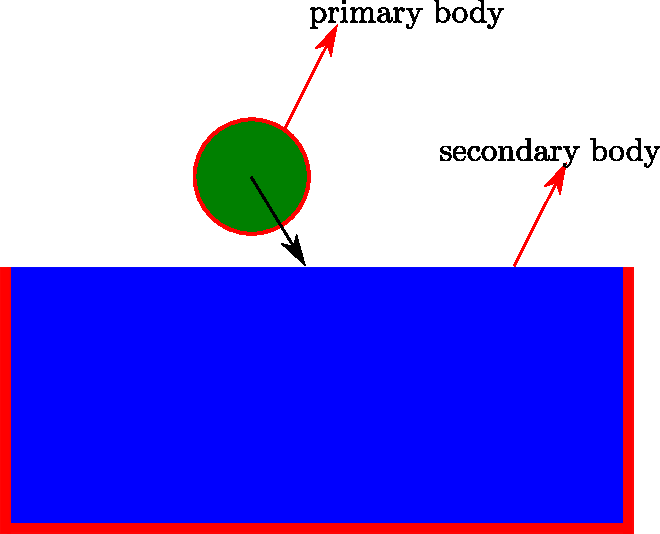
\includegraphics[width=0.5\textwidth]{images/erosion/images/contact_force/contact_force_divide}
  \caption{Bodies under collision which are divided into primary and
    secondary.}
\label{fig:erosion-cnt-force-divide-bodies}
\end{figure}

Force on the particle $i$ of elastic-plastic structure is computed as,


% Which body is considered primary and secondary

% ====================================================================================
% ====================================================================================
\FloatBarrier%
\section{Result: A rigid sphere hitting a ductile specimen at different impact velocities}
\label{sec:r-vyas}
\begin{figure}[!htpb]
  \centering
  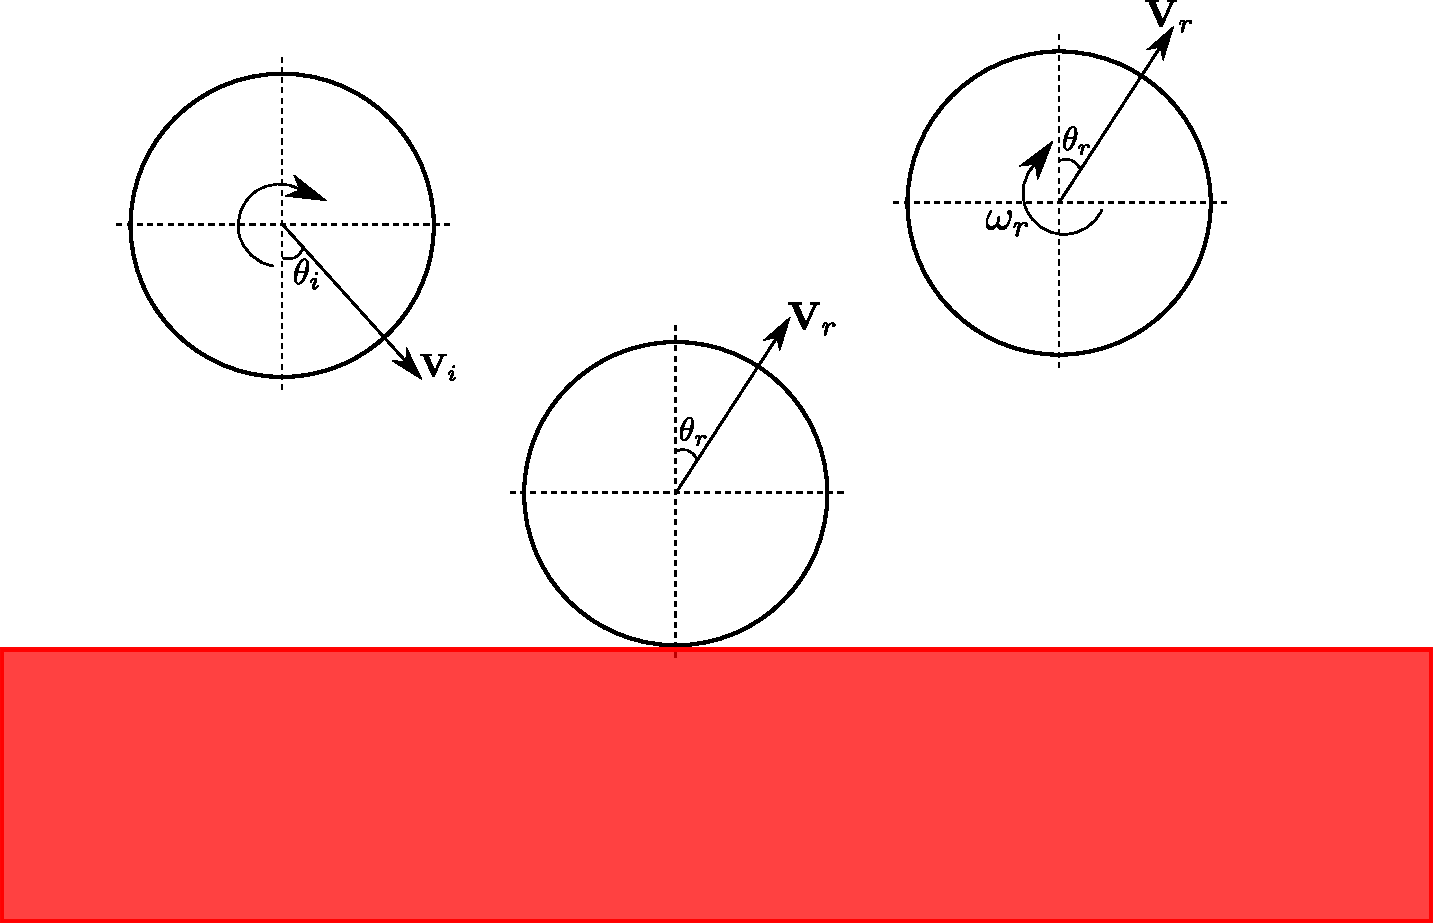
\includegraphics[width=0.6\textwidth]{images/erosion/images/vyas_2021_rebound_kinematics_3d/cao_drawing}
  \caption{A spherical particle impacting a ductile target at an impact angle
    with a velocity $\ten{V}_i$.}
\label{fig:results-cao-3d-erosion-schematic}
\end{figure}
In the current example, we simulate the impact of a 3D sphere on a wall at
different impact velocities, where the experimental evaluation is done by
\cite{zang2022investigation}. The model description is shown in
\cref{fig:results-cao-3d-erosion-schematic}. The sphere is assumed to be
rigid and the material properties as well as the numerical parameters used are
displayed in \cref{tab:sphere-target-impact}. The sphere is impacted on the wall
by varying the incident velocities ($\ten{V}_i$) keeping the incident angle constant,
$45$ degrees.
\begin{table}[!ht]
  \centering
  \begin{tabular}[!ht]{ll}
    \toprule
    Quantity & Values\\
    \midrule
    $E$, Young's modulus & $70$ GPa \\
    $\nu$, Poisson's ratio & $0.33$ \\
    $\rho$, density & $2700$ kg\,m\textsuperscript{-3} \\
    $\mu$, friction coefficient & $0.1$ \\
    Time of simulation & $0.25$ ms \\
    Resolution, $\delta x$ & $0.00153$ m\\
    Smoothing length factor, $h/\Delta x$ & 1.0\\
    gravity $[g_x, g_y, g_z]$ & $[0.0, -9.81, 0.0]$\\
    $k_r$, Normal stiffness coefficient & $10^{7}$ \\
    $k_f$, Tangential stiffness coefficient & $10^{5}$ \\
    $\text{Radius}$, Sphere radius & 5 $\times$ $10^{-3}$ m\\
    \bottomrule
  \end{tabular}
  \caption{Numerical parameters and material properties for sphere impacting a target.}%
  \label{tab:sphere-target-impact}
\end{table}



\begin{table}[!ht]
  \centering
  \begin{tabular}[!ht]{ll}
    \toprule
    Quantity & Values\\
    \midrule
    $A$ & $335$ MPa \\
    $B$ & $85$ MPa \\
    $C$ & $0.012$ \\
    $m$ & $1$ \\
    $n$ & $0.11$ \\
    $T_{ref}$ & $292$K \\
    $T_{melt}$ & $925$K \\
    \bottomrule
  \end{tabular}
  \caption{Johnson-Cook constitutive model parameters for the target.}%
  \label{tab:sphere-target-impact-Johnson}
\end{table}
\begin{figure}[!htpb]
  \centering
  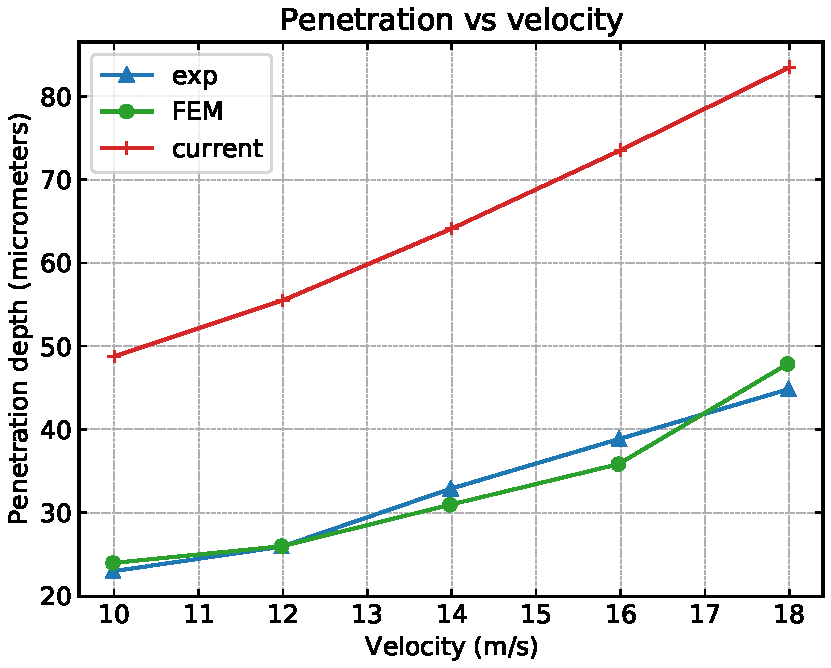
\includegraphics[width=0.6\textwidth]{figures/erosion/figures/cao_xuerui_2022_spherical_particle_impact_3d/penetration_vs_velocity}
  \caption{Variation of the penetration depth with the varying incident velocity
    magnitude compared against the experimental and numerical study with the
    current solve.}
  \label{fig:results-sphere-target-impact-vel-vs-depth}
\end{figure}
\Cref{fig:results-sphere-target-impact-vel-vs-depth} depicts the variation of
the depth against the incident velocity $\ten{V}_i$. The simulated results are
compared to the experimental results by \cite{zang2022investigation} as well as
the computational results simulated using finite element method modeling. We
wish to complete this problem till the time of thesis submission.
